 \documentclass[final,3p,times,onecolumn,sort&compress,hidelinks]{elsarticle}


%% Use the options 1p,twocolumn; 3p; 3p,twocolumn; 5p; or 5p,twocolumn
%% for a journal layout:
%% \documentclass[final,1p,times]{elsarticle}
% \documentclass[final,1p,times,twocolumn]{elsarticle}
%% \documentclass[final,3p,times]{elsarticle}
%% \documentclass[final,3p,times,twocolumn]{elsarticle}
%% \documentclass[final,5p,times]{elsarticle}
%% \documentclass[final,5p,times,twocolumn]{elsarticle}

%\documentclass[final,5p,times,twocolumn,sort&compress]{elsarticle}


%\documentclass[final,1p,times,twocolumn]{elsarticle}
%\documentclass[3p,10pt]{elsarticle}

%----------------------------------------------------------------
\usepackage[normalem]{ulem}
\usepackage[utf8]{inputenc}
%\usepackage{kantlipsum}
%\usepackage{lipsum,widetext}
\usepackage{slashed}
\usepackage{graphicx}
\usepackage{hyperref}
\usepackage{bm}
\usepackage[usenames]{color}
\usepackage{listings}
\usepackage{pdfpages}
\usepackage{pstricks}
%\usepackage{cite}
\usepackage{color}
\usepackage{enumerate}
\usepackage{float}
\usepackage{amsmath}
\usepackage{amssymb}
\usepackage{mathtools}
\usepackage{amssymb}
\usepackage{marvosym}
%\usepackage[OT2,T1]{fontenc}
%----------------------------------------------------------------
%\DeclareSymbolFont{cyrletters}{OT2}{wncyr}{m}{n}
%\DeclareMathSymbol{\Sha}{\mathalpha}{cyrletters}{"58}
\newcommand{\question}[1]{\underline{\textcolor{red}{Question:}}{\; #1}}
\newcommand{\nf}[2]{#1_{#2,R}}
\newcommand{\Tsc}[2]{#1_{#2\text{T}}}
\newcommand{\Tscsq}[2]{#1^2_{#2\text{T}}}
\newcommand{\hadp}{{\ensuremath{{\bf P}_h}}}
\newcommand{\hadpsc}{{\ensuremath{P_h}}}
\newcommand{\hadmass}{\ensuremath{M_h}}
\newcommand{\qmass}{\ensuremath{m_q}}
\newcommand{\bquote}[1]{\textcolor{blue}{ \begin{quote} ``#1'' \end{quote}}}
\newcommand{\T}[2]{\boldsymbol{#1}_{#2\text{T}}}
\newcommand{\nft}[2]{#1_{#2\text{T},R}}
\newcommand{\nftb}[2]{\boldsymbol{#1}_{#2\text{T},R}}
\newcommand{\cs}[2]{ \Gamma^{#2}(\Tsc{q},Q_{#1}) }
\newcommand{\csb}[2]{ \tilde{\Gamma}^{#2}(\Tsc{b},Q_{#1}) }
\newcommand{\as}[2]{{\rm AY}^{#2}(\Tsc{q}{},Q_{#1})}
\newcommand{\asnew}[2]{{\rm AY}_{\rm New}^{#2}(\Tsc{q},Q_{#1};\eta,C_5)}
\newcommand{\fixo}[2]{{\rm FO}^{#2}(\Tsc{q}{},Q_{#1})}
\newcommand{\TT}[2]{W^{#2}(\Tsc{q},Q_{#1})}
\newcommand{\TTnew}[2]{W_{\rm New}^{#2}(\Tsc{q},Q_{#1};\eta,C_5)}
\newcommand{\TTa}[2]{W_{\rm a}^{#2}(\Tsc{q},Q_{#1};\eta,C_5)}
\newcommand{\TTb}[2]{\Tilde{W}^{#2}(\Tsc{b},Q_{#1})}
\newcommand{\YY}[2]{Y^{#2}(\Tsc{q},Q_{#1})}
\newcommand{\YYnew}[2]{Y_{\rm New}^{#2}(\Tsc{q},Q_{#1};\eta,C_5)}
%\newcommand{\no}{\nonumber \\}
\newcommand{\bmax}{b_{\rm max}}
\newcommand{\bmin}{b_{\rm min}}
%\newcommand{\bss}{\color{blue}b_{1*}}
%\newcommand{\bss}{\odot}
\newcommand\bstar{\3{b}_*}
\newcommand\bstarsc{b_*}
\newcommand\bbar{\bar{b}}
\newcommand{\parz}[1]{\ensuremath{\left(#1\right)}}
\newcommand\qstar{\Tsc{q}^*}
\newcommand\bone{b_c}
\newcommand\mubstar{\mu_{\bstarsc}}
\newcommand\muQ{\mu_Q}
\newcommand{\Qin}{Q_{\rm init}}
\newcommand{\appor}[1]{{\rm T}_{\rm #1}}
\newcommand\bstarstar{\3{b}_{**}}
\newcommand\mub{\mu_b}
\newcommand{\bT}{\3{{b}_T}}
\newcommand{\wvar}{\text{\Leo}}
\newcommand{\wwvar}{\text{\Saturn}}
\newcommand{\mucirc}{\bar{\mu}}
\newcommand{\mucircm}{\mu_c}
\newcommand{\jbar}{\bar{\jmath}}
\newcommand{\nc}{\frac{1}{N_{\rm c}}}
%\newcommand{\nc2}{\frac{1}{N_{\rm c}^{2}}}
%\newcommand{\nc3}{\frac{1}{N_{\rm c}^{3}}}
\newcommand{\nctmo}{\frac{1}{N_c^2-1}}
\newcommand{\ths}{\hat{s}}
\newcommand{\tht}{\hat{t}}
\newcommand{\thu}{\hat{u}}
\newcommand{\parr}{\left(x\thu+x^\prime\tht\right)}

\DeclareRobustCommand*\diff[2][]{%
   \mathop{
     \mathrm{d}^{#1}
     \mskip-0.2\thinmuskip
    #2}\nolimits
}
\usepackage{soul}

%%%%%%%%%%%%%%%%%%%%%%%%%%%%%%%%%%%%%%%%%%%%%%%%%%%%%%%%%%%%%%%%%%%%%%%%
%% june 9, 2016:
%%%%%%%%%%%%%%%%%%%%%%%%%%%%%%%%%%%%%%%%%%%%%%%%%%%%%%%%%%%%%%%%%%%%%%%%
%\documentclass[floatfix,aps,prd,nofootinbib,superscriptaddress,preprint]{revtex4}
%\pdfoutput=1
%\extrafloats{100}
%%%%%%%%%%%%%%%%%%%%%%%%%%%%%%%%%%%%%%%%%%%%%%%%%%%%%%%%%%%%%%%%%%%%%%%%
\usepackage{amsmath,amssymb}
\usepackage{bm,bbm}
\usepackage{graphicx, graphics, color}
\usepackage{slashed}
\usepackage{booktabs}
%\usepackage{tabu}
%\usepackage[dvipsnames]{xcolor}
%
%%%%%%%%%%%%%%%%%%%%%%%%%%%%%%%%%%%%%%%%%%%%%%%%%%%%%%%%%%%%%%%%%%%%%%%%
% macros for labeling
%%%%%%%%%%%%%%%%%%%%%%%%%%%%%%%%%%%%%%%%%%%%%%%%%%%%%%%%%%%%%%%%%%%%%%%%
% shorcuts 

%\documentclass[prd,preprintnumbers,nofootinbib,superscriptaddress]{revtex4-1}
%\pdfoutput=1
%\usepackage{graphicx}
%\usepackage{amsmath}
%\usepackage{amssymb}
%\usepackage{mathtools}
%\usepackage[bookmarksopen,bookmarksnumbered]{hyperref}
%\usepackage{color}
%\usepackage[usenames,dvipsnames]{xcolor}
%\usepackage[normalem]{ulem}
%\usepackage{soul}
%\usepackage{units}
%\usepackage{rotating}

\allowdisplaybreaks

% Define \xleft to be like \left except to produce spacing suitable
% for the opening parenthesis of a function argument:
\def\xleft{\mathopen{}\left}

\newcommand\3[1]{\boldsymbol{#1}}

% Transverse component of vector
% Extra {} gets subscript 'T's to line up, as in \T{y}-\T{z}

% Notation for asymptote
\def\asy{\mathop{\text{asy}}}

\newcommand\BIBjour[1]{\emph{#1}}
\newcommand\BIBvol[1]{\textbf{#1}}

% bstar, etc (for TMD functions)
\newcommand{\crd}{\color{red}}
\newcommand{\cbl}{\color{blue}}
\newcommand{\cma}{\color{magenta}}
\newcommand{\no}{\nonumber \\}
\newcommand{\bss}{\odot}
\newcommand\pORm[2]{\genfrac{}{}{0pt}{2}{+#1}{-#2}}

\newcommand{\bea}{\begin{eqnarray}}
\newcommand{\eea}{\end{eqnarray}}
\newcommand{\nn}{\nonumber}
\newcommand{\ben}{\begin{eqnarray}}
\newcommand{\ee}{\end{equation}}
\newcommand{\een}{\end{eqnarray}}
\newcommand{\nnu}{\nonumber\\}



\newcommand*{\FigPath}{../Figs/}%  


%%%%%%%%%%%%%%%%%%%%%%%%%%%%%%%%%%%%%%%%%%%%%%%%%%%%%%%%%%%%%%%%%%%%%%%%
\begin{document}
\begin{flushleft}
%%%%%%%%%%%%%%%%%%%%%%%%%%%%%%%%%%%%%%%%%%%%%%%%
%\begin{figure}[h]
%\includegraphics[width=.2\textwidth]{\FigPath/tmd_collaboration.pdf}
%\vspace{0.5cm}
%\end{figure}
%%%%%%%%%%%%%%%%%%%%%%%%%%%%%%%%%%%%%%%%%%%%%%%%%
\end{flushleft}
\vspace{-3.0cm}
\begin{flushright}
JLAB-XXXX
\vspace{0.5cm}
\end{flushright}

\begin{frontmatter}

\author{Mason Albright\fnref{label1}}
\author{Scott Dolan\fnref{label1}}
\author{Leonard Gamberg\fnref{label2}}
\author{Wally Melnitchouk\fnref{label3}}
\author{\\Daniel Pitonyak\fnref{label2}}
\author{Alexei Prokudin\fnref{label2,label3}} 
\author{Nobuo Sato\fnref{label3}}
\author{Zackary  Scalyer\fnref{label4}}
\address[label1]{College of Engineering, Penn State University, State College, Pennsylvania 16801, USA}
\address[label4]{Dipartimento di Fisica Teorica, Universit$\grave{a}$ di Torino, Via P. Giuria 1, I-10125 Torino, Italy}
\address[label5]{Dipartimento di Fisica, Universit$\grave{a}$ di Cagliari, Cittadella Universitaria, I-09042 Monserrato
(CA), Italy}
\address[label2]{Division of Science, Penn State University Berks, Reading, Pennsylvania 19610, USA}
\address[label3]{Theory Center, Jefferson Lab, 12000 Jefferson Avenue, Newport News, Virginia 23606, USA}
\address[label4]{?}


\title{Study of collinearity criteria and unpolarized Transverse Momentum Dependent distributions using HERMES multiplicities in semi-inclusive deep-inelastic scattering}


%%%%%%%%%%%%%%%%%%%%%%%%%%%%%%%%%%%%%%%%%%%%%%%%%%%%%%%%%%%%%%%%%%%%%%%%
\begin{abstract}
  We analyze HERMES multiplicities in semi-inclusive deep-inelastic scattering and extract non-perturbative transverse momentum dependence of unpolarized transverse momentum dependent distributions. We discuss the importance of data selection in conducting the fits of the multiplicities.  In particular
  we implement   the  collinearity criteria introduced in reference~\cite{Boglione:2016bph} that allow us to study the effects of selecting data
  that is  predominantly in the current fragmentation region.  We compare our parameters to previous extractions in order to better interpret our results.  We also give an outlook on what impact this criteria can have for on-going and future experiments.
\end{abstract}



\begin{keyword}
unpolarized TMDs \sep semi-inclusive deep-inelastic scattering \sep perturbative QCD

\PACS 12.38.-t \sep 12.38.Bx \sep  13.85Fb \sep 13.85.Ni \sep 13.87Fh

%% MSC codes here, in the form: \MSC code \sep code
%% or \MSC[2008] code \sep code (2000 is the default)

\end{keyword}

\end{frontmatter}


\date{\today}



\section{Introduction}
\label{s:intro}
Understanding the internal structure of hadrons has been a topic of intense research for over 50 years.  From inclusive and semi-inclusive deep inelastic scattering (DIS) experiments, we know that hadrons  have a complex internal structure
composed of quarks, anti-quarks, and gluons (partons). In addition to the parton's  collinear momentum, which is highly correlated  with the direction of a fast-moving parent hadron, they 
have intrinsic transverse motion and structure. Several types of DIS experiments are sensitive to this intrinsic momentum structure: semi-inclusive deep-inelastic scattering (SIDIS) ($e\,N\to e'\,h\,X$)~\cite{Kotzinian:1994dv}, electron-positron annihilation to almost back-to-back hadrons ($e^+e^-\to h_a\,h_b\,X$)~\cite{Boer:1997mf}, and Drell-Yan ($p\,p\to l^+\,l^-\,X$)/weak gauge boson production ($p\,p\to \{Z, W^+, W^-\}\,X$)~\cite{Tangerman:1994eh}. To connect these measurements  to a theoretical framework, 
one relies on QCD factorization theorems where
TMD factorization~\cite{Collins:1981uw,Ji:2004wu,Collins:2011zzd}
describes these DIS processes in terms of  a collinear perturbative (hard) scattering cross section and  non-perturbative 
transverse momentum dependent (TMD)
 parton distribution functions (PDFs) and fragmentation functions (FFs) (collectively called TMDs)~\cite{Kotzinian:1994dv,Mulders:1995dh,Boer:1997nt}. 

\begin{flushleft}
{\em [Discussion on what was done in the past (i.e., Berger criteria $\to$ ``standard'' cut).]}
\end{flushleft}
 
 A condition implicit in the proofs of TMD factorization in SIDIS,
 where hadrons are detected in the final state as fragments of the
 struck quark, the assumption of  a clear separation in momentum of the struck quark from the target spectators.  Then it is natural to conclude that the fragmentation of the quark into hadrons is independent of the production of the quark~\cite{Berger:1987zu,Mulders:2000jt,Joosten:2013mia}. This picture
 implies that fragmentation can be described by a function of $z$ independent of $x$~\cite{Berger:1987zu}.  By contrast if the produced hadron moves in nearly the same direction as the target then the hadron is said to be in the target fragmentation region and the relevant factorization theorem uses fracture functions~\cite{ Trentadue:1993ka,Grazzini:1997ih,Anselmino:2011ss}.  
 A clear distinction between the current and target  region, require large enough separation in momentum of the current and target fragments.  It has proved  convenient to use rapidity to delineate these regions.   Some time ago Berger provided a rapidity gap criteria  to study the dynamics of quark fragmentation in the current region~\cite{Berger:1987zu,Mulders:2000jt}.  In reality the classification of distinct current, target, and central fragmentation regions however, are not sharp~\cite{Berger:1987zu,Mulders:2000jt,Joosten:2013mia,Boglione:2016bph,Collins:2018teg}.

 Recently, it has been shown that at moderate to low values of $Q$, estimating the adequacy of the current fragmentation criteria requires knowledge of intrinsic non-perturbative properties of partons. That analysis depends on a close examination of the errors in TMD factorization, resulting in
 a more restrictive region where current fragmentation by itself is valid~\cite{Boglione:2016bph}.
 %as those in SIDIS experiments the distinction between these regions becomes blurred~\cite{Boglione:2016bph}.
   Additionally it was pointed out that the applicability of TMD factorization, that is factorization  with fragmentation in  current region, not only depends on a clearly separate and relatively distinct target and current rapidity regions but also depends on the transverse momentum of the current hadron, $P_{hT}$ ({\em we should be clear about using $q_T$ and or $P_{hT}$ re: $z_h$ : see Sec. 3.1})  
 to study this issue.  Indeed, recent work shows that for these SIDIS experiments, the standard cuts~\cite{Anselmino:2013lza} (more references to fits Bacchetta et al. \dots)
   are not enough, and the current and target fragmentation regions may overlap, to the point where certain kinematic bins thought to be in the current regime are actually in the target sector~\cite{Boglione:2016bph}.  In principle, this mixing of hadrons produced from the target, central and current region can affect the extraction of TMDs and interpretation of the fitted functions.
  Therefore, it is of utmost importance to analyze the impact of cuts separating current from target and central fragmentation regions on the extraction of TMDs in order to better improve the phenomenology moving forward.

\begin{flushleft}  
  {\em A lines or two more on the collinearity criteria $\rightarrow$ R-cut/filter as an introduction and continue in Section 3.1}.
  \end{flushleft}

  
In this Letter, we  implement for the first time the collinearity criteria~\cite{Boglione:2016bph} in an extraction of TMD widths for unpolarized PDFs and FFs.  In order to avoid issues with evolution, we focus only on HERMES multiplicity data in SIDIS.  We use a simple analytical approximation for the solutions of TMD evolution equations that is valid in the non-perturbative region and  extract transverse momentum dependence of TMDs allowing the widths to vary with flavor.  The Letter is organized as follows: in Sec.~\ref{s:model} we summarize the theoretical formalism needed to analyze the data, including our model for the transverse momentum dependence.  Next, in Sec.~\ref{s:phenom} we give details on our data selection and perform our fit of the HERMES multiplicities in order to extract the relevant TMD widths.  We also compare our results with previous works and give an interpretation of our widths in the context of these other extractions.  Finally, in Sec.~\ref{s:concl} we summarize our findings and give an outlook on the impact of this analysis for on-going and future experiments.



\section{Theoretical Formalism}
\label{s:model}
Consider the process of SIDIS off an unpolarized nucleon target $N=p,n,d,...$,
\begin{equation}
\ell(l)+p(N)\to \ell'(l') + h(P_h) + X\,,
\end{equation}
where the momenta of the particles are given, and we consider only the exchange of a single virtual photon $\gamma^*(q)$.  One can define the standard Lorentz invariants for this reaction as
\begin{equation}
S = (l+P)^2\,, \quad\quad Q^2 = -q^2 = -(l-l')^2\,, \quad\quad x_B = \frac{Q^2} {2P\cdot q}\,, \quad\quad y = \frac{Q^2} {x_B S}\,, \quad\quad z_h = \frac{P\cdot P_h} {P\cdot q}\,.
\end{equation}
One also often uses a vector $\vec{q}_T \simeq -\vec{P}_{hT}/z$ as far as applicability region of TMD factorization~\cite{Collins:2011zzd} is proven to be $q_T \ll Q$.
For the situation where $q_{T}\ll Q$, one finds at leading-order~\cite{Bacchetta:2006tn}
\begin{eqnarray}
\frac{d\sigma}
{dx_B\, dQ^2 \, dz_h \, dP_{hT}^2} &\!\!\!=\!\!\!&
\frac {2 \, \pi^2 \alpha_{em}^2}{(x_B S)^2} \, \frac{ 1 + (1-y)^2 }{y^2}\,F_{UU}(x,z,P_{hT}^2,Q^2) + \mathcal{O}(q_{T}/Q)
\label{e:dsigma}
\end{eqnarray}
where \cite{Collins:2011zzd}
\begin{equation}
F_{UU}(x,z,P_{hT}^2,Q^2)  = {\cal H} (Q; \mu_Q)\sum_{a} e_a^2 \,
\int d^2\vec{k}_\perp \, d^2\vec{p}_\perp
\> \delta ^{(2)}\Big(\vec{P}_{hT} - z_h\,\vec{k}_\perp -\vec{p}_\perp\Big)\,
f_{a/N} (x, k_{\perp}; Q^2, \mu_Q) \, D_{h/a}(z, p_{\perp}; Q^2, \mu_Q)\,. \label{e:FUU} \\
\end{equation}
The functions $f_{a/N} (x, k_{\perp}; Q^2, \mu_Q)$ and $D_{h/a}(z, p_{\perp}; Q^2, \mu_Q)$ are the unpolarized TMD PDF and FF, respectively, for a parton of flavor $a$~\cite{Bacchetta:2006tn,Collins:2011zzd}.  The function ${\cal H}$ is the so-called hard function, we will use the $0^{th}$ order of ${\cal H} = 1$. In the $\gamma^*$-$p$ center-of-mass frame, we have the following relations up to $\mathcal{O}(q_{T}/Q)$ and $\mathcal{O}(M_N/Q)$ corrections~\cite{Bacchetta:2006tn}
\begin{equation}
 x=x_B\,, \quad\quad z=z_h\,,\label{e:LT_relations}
\end{equation}
Apart from kinematical variables and transverse momentum TMD functions depend on the scale of the reaction, $Q^2$.
The dependence of functions $f_{a/N} (x, k_{\perp}; Q^2, \mu_Q)$ and $D_{h/a}(z, p_{\perp}; Q^2, \mu_Q)$  on the scale $Q^2$ is encoded in solutions of Collins-Soper (CS) evolution equations~\cite{Collins:2011zzd} in Fourier conjugate to $k_{\perp}$ space $b_T$. In this analysis we study the separation of beam and target fragmentation regions and we need an analytical form of TMDs in the momentum space in order to speed up our numerical calculations, thus we will utilize an estimate for the solution of CS equations that is valid in non-perturbative region corresponding to large $b_T$ or small $k_\perp$. We will start from the solution of CS equations from Ref.~\cite{Collins:2014jpa} at a given fixed scale, $Q_0=\mu_0$:
\begin{eqnarray}
&&\tilde f_{a/N} (x,b_T; Q^2, \mu_Q)= \tilde f_{a/N} (x, b_T; Q_0^2, \mu_0)\,e^{-S(b_T, Q, \mu_Q, Q_0, \mu_0)/2}\,,
\label{e:PDF_ansatz}\\[0.3cm]
&&\tilde D_{h/a}(z,b_T; Q^2, \mu_Q)=\frac{1}{z^2}\tilde D_{h/a}(z, b_T; Q_0^2, \mu_0)\,e^{-S(b_T, Q, \mu_Q, Q_0, \mu_0)/2}\,,
\label{e:FF_ansatz0}
\end{eqnarray}
where $b_T$ is Fourier conjugate variable to $k_\perp$; $Q_0$ and $\mu_0$ are chosen fixed reference scales (we will choose $\mu_0 = Q_0$). The evolution factor is $e^{-S(b_T, Q, Q_0, \mu_0)/2}$, where
\begin{eqnarray}
S(b_T, Q, \mu_Q, Q_0, \mu_0) = \tilde K(b_T,\mu_0) \ln\frac{Q^2}{Q_0^2} - \int_{\mu_0}^{\mu_Q} \frac{d \mu'}{\mu'}\left[
-2 \gamma_i(\alpha_s(\mu');1) +\ln\frac{Q^2}{\mu'^2}\gamma_K(\alpha_s(\mu'))\,,
 \right]
 \label{e:FF_ansatz}
\end{eqnarray}
where $\tilde K$ is the so-called Collins-Soper evolution kernel, $\gamma_i$ and $\gamma_K$ are anomalous dimensions of the TMD and $\tilde K$ accordingly and can be calculated perturbatively provided $\alpha_s$ is small enough. We will choose $\mu_Q = Q$. 

The next step is to choose $b_T$ parameterization of TMDs at the initial scale $Q_0$. In this study the parameterization can be chosen arbitrary provided an analytical FT transform is possible for the sake of numerical computation speed. Low $Q^2$ data is known \cite{Schweitzer:2010tt} to have an approximate Gaussian dependence and we will follow a very simple analytical form used in Refs~\cite{Anselmino:2013lza,Signori:2013mda}, and choose a Gaussian ansatz for $b_T$ dependence (note that we also allow for a flavor dependence in the widths of the Gaussians):
\begin{eqnarray}
&&\tilde f_{a/N} (x,b_T; Q_0^2, \mu_0)\simeq f_{a/N} (x; Q_0^2, \mu_0) e^{-b_T^2 \frac{\langle k_\perp^2 \rangle_a}{4}}\,,
\nonumber \\[0.3cm]
&&\tilde D_{h/a}(z,b_T; Q_0^2, \mu_0)\simeq \frac{1}{z^2} D_{h/a}(z; Q_0^2, \mu_0) e^{-b_T^2 \frac{\langle p_\perp^2 \rangle_a}{4 z^2}}.
\label{e:FF_ansatz1}
\end{eqnarray}
The parameterizations in Eqs.~\eqref{e:FF_ansatz1} are chosen in such a way that we can make a connection of $\tilde f_{a/N} (x; Q_0^2, \mu_0)$ and $\tilde D_{h/a}(z; Q_0^2, \mu_0)$ to the usual collinear PDF and FF functions. Indeed, using result of Ref.~\cite{Collins:2016hqq} we know that at leading order in $\alpha_s$, the collinear integrated cross-section corresponds to the integral in $P_{hT}$ of the TMD approximated cross-section. Using $S(b_T, Q_0, \mu_0, Q_0, \mu_0) = 0$ we obtain:
\begin{eqnarray}
&&\tilde f_{a/N} (x; Q_0^2, \mu_0) = f_{a/N} (x, Q_0)\,,
\\[0.3cm]
&&\tilde D_{h/a}(z; Q_0^2, \mu_0) = D_{h/a}(z, Q_0)\,,
\label{e:FF_ansatz2}
\end{eqnarray}
where $f_{a/p} (x, Q_0)$ and $D_{h/a}(z, Q_0)$ are the standard unpolarized collinear PDF and FF, respectively, for a parton of flavor $a$, at the initial scale.

Using a typical value of $\langle k_\perp^2 \rangle = 0.25$ (GeV$^2$) \cite{Anselmino:2005nn} for the width of TMDs we can easily show in Fig.~\ref{Fig:width} $b_T$ behavior of unpolarized TMDs at initial scale $Q_0$.

Let us denote
\begin{eqnarray}
S_{pert} \equiv \int_{\mu_0}^{\mu_Q} \frac{d \mu'}{\mu'}\left[
-2 \gamma_i(\alpha_s(\mu');1) +\ln\frac{Q^2}{\mu'^2}\gamma_K(\alpha_s(\mu'))
 \right] \; ,
 \label{e:FF_Spert}
\end{eqnarray}
and using the first loop results for $\gamma_i$ and $\gamma_K$ for from Ref.~\cite{Aybat:2011zv}, we have:
\begin{eqnarray}
\gamma_K(\alpha_s(\mu')) = 2 C_F \frac{\alpha_s}{\pi} \, ,  \;
\gamma_i(\alpha_s(\mu');1) = 2 C_F \frac{\alpha_s}{\pi} \frac{3}{2} \, ,\\
S_{pert} = 2 C_F \int_{\mu_0}^{\mu_Q} \frac{d \mu'}{\mu'} \frac{\alpha_s(\mu')}{\pi} \left[\ln\frac{Q^2}{\mu'^2} - \frac{3}{2}
 \right] \; ,
 \label{e:FF_Spert1}
\end{eqnarray}
where $C_F = 4/3$. In order to calculate analytically the integral from Eq.~\eqref{e:FF_Spert1} we will use the first loop result for the strong coupling constant:
\begin{eqnarray}
\alpha_s(\mu') = \frac{1}{\beta_0 \ln Q^2/\Lambda^2} \; , \quad\quad
\beta_0 = \frac{33-2 n_f}{12 \pi}\; ,
 \label{e:as}
\end{eqnarray}
where we will use $n_f=3$ as we are interested in the region of low Q; and $\Lambda = 0.25$ (GeV), such that $\alpha_s(M_Z)= 0.118$ ~\cite{Bethke:2012jm}. We obtain, see also Ref.~\cite{Aidala:2014hva}:
\begin{eqnarray}
S_{pert} = -\frac{2 C_F}{\pi \beta_0}\left ( \ln \frac{Q}{Q_0} - \ln \frac{Q}{\Lambda} \ln \left(\frac{\ln \frac{Q}{\Lambda}}{\ln \frac{Q_0}{\Lambda}} \right)+
\frac{3}{4} \ln \left(\frac{\ln \frac{Q}{\Lambda}}{\ln \frac{Q_0}{\Lambda}} \right)\right).
 \label{e:FF_Spert_analytical}
\end{eqnarray}

We will assume that the functional form of TMDs in $b_T$ space is such that {\em only} large values of $b_T$  dominate in the FT connecting momentum and coordinate spaces and will approximate $K(b_T,\mu_0)$ by its large $b_T$ asymptotic: a constant, as suggested in Ref.~\cite{Collins:2014jpa}. We will
call this constant $g_{K_0}\equiv \lim_{b_T\to \infty} \tilde K(b_T,\mu_0)$, such that in this approximation
\begin{eqnarray}
&&\tilde f_{a/p} (x,b_T; Q^2, \mu_Q)\simeq \tilde f_{a/p} (x, b_T; Q_0^2, \mu_0)\,\left( \frac{Q}{Q_0}\right)^{g_{K_0}} e^{-S_{pert}/2}\,,
\nonumber \\[0.3cm]
&&\tilde D_{h/a}(z,b_T; Q^2, \mu_Q)\simeq \frac{1}{z^2}\tilde D_{h/a}(z, b_T; Q_0^2, \mu_0)\,\left( \frac{Q}{Q_0}\right)^{g_{K_0}}e^{-S_{pert}/2}\,.
\label{e:FF_ansatz1}
\end{eqnarray}
Our result suggests that in the region of its applicability TMD evolution accounts to the shift of normalization in $Q^2$ and does not lead to the usual broadening of TMDs observed~\cite{Collins:2011zzd} at large $Q^2$. This result is consistent with the experimental findings \cite{Airapetian:2012ki} of HERMES collaboration: no significant broadening of multiplicities was observed as a function of $Q^2$. Notice that our approximation of $K(b_T,\mu_0)$ is a very crude one, so we do not expect the result to hold generically; in particular, it will fail at large $Q^2$ where low values of $b_T$ dominate in the FT. This simplification is taken deliberately to be able to speed up the numerical computations, otherwise  a specific functional form of $\tilde K(b_T,\mu_0)$ should be used and it should satisfy the following criteria:
$\lim_{b_T\to \infty} \tilde K(b_T,\mu_0) = const$, $\lim_{b_T\to 0} \tilde K(b_T,\mu_0) = 0$. Ref.~\cite{Collins:2014jpa} suggests high $b_T$ limit of $\tilde K(b_T,\mu_0)$ should be negative, we will be able to phenomenologically test this assumption.


Finally we arrive at the following parameterization of the unpolarized structure function from Eq.~(\ref{e:FUU}) 
\begin{equation}
F_{UU}(x_B,z_h,P_{hT}^2,Q^2)  =  \sum_{a} \, e_a^2 \,f_{a/p}(x_B, Q_0)\,D_{h/a}(z_h, Q_0) \left( \frac{Q^2}{Q_0^2}\right)^{g_{K_0}}e^{-S_{pert}}\,
\frac{e^{-P_{hT}^2/\langle P_{hT}^2 \rangle_a}}{\pi\langle P_{hT}^2 \rangle_a}\,, \label{e:FUU_model}
\end{equation}
with
\begin{equation}
\langle P_{hT}^2 \rangle_a = \langle p_\perp^2 \rangle_a + z_h^2\, \langle k_\perp^2 \rangle_a\,, \label{e:avg_kT}
\end{equation}
where we have used the expressions from Eq.~(\ref{e:LT_relations}).  
Notice that our result is similar to Refs.~\cite{Anselmino:2013lza,Signori:2013mda}, with the following important differences:
We do not utilize DGLAP evolution for TMDs as was done in Ref.~\cite{Anselmino:2013lza} and we do not freeze the scale either as was done in Ref.~\cite{Signori:2013mda}. We mention that a fit of HERMES~\cite{Airapetian:2012ki}  and COMPASS~\cite{Adolph:2013stb} multiplicities with full TMD evolution and next-to-leading logarithmic accuracy was published in Ref.~\cite{Bacchetta:2017gcc}. In this study we do not aim at a complete fit of the data at different $Q^2$ and choose to fit only HERMES~\cite{Airapetian:2012ki} multiplicities. Our result is consistent with CS equations, provided that the scale $Q$ is not drastically different from $Q_0$ and TMDs are dominated by the region of large $b_T$, so that $\tilde K(b_T,\mu_0)$ is approximately constant.

From this, we find our formula for the HERMES multiplicities~\cite{Airapetian:2012ki} 
\begin{equation}
M_n^h(x_B, Q^2,z_h, P_{hT}) =
2P_{hT}\frac{\pi\, \sum_{a} e_a^2 \,f_{a/p}(x_B, Q_0)\,D_{h/a}(z_h, Q_0)}
{\sum_{a} e_a^2 \> f_{a/p} (x_B,Q^2)} \,  \left( \frac{Q^2}{Q_0^2}\right)^{g_{K_0}}e^{-S_{pert}}\,
\frac{e^{-P_{hT}^2/\langle P_{hT}^2 \rangle_a}}{\pi\langle P_{hT}^2 \rangle_a}
\,. \label{e:mult_HERMES}
\end{equation}


\section{Phenomenological Analysis and Discussion}
\label{s:phenom}

\subsection{Data Selection}
\label{s:data}
Prior to performing a fit of an experimental measurement, one often needs to make cuts on the data to ensure that the fit is restricted only to the data that can be described by the theoretical model.  For example, a ``standard'' cut on the HERMES multiplicity data is~\cite{Anselmino:2013lza}
\begin{equation}
z_h < 0.6 \quad\quad Q^2 > 1.69 \; \textrm{GeV}^2  
\quad\quad 0.2 < P_{hT} < 0.9 \; \textrm{GeV} \quad\quad\quad{\rm (standard\;cut)}\,.\label{e:st_cut}
\end{equation}
However, as was argued in Ref.~\cite{Boglione:2016bph}, Eq.~(\ref{e:st_cut}) is not sufficient to guarantee that one stays strictly in the current (or the so-called ``beam") fragmentation region.  Instead, one should calculate the ratio $R(y_h,z_h,x_B,Q)$, called the collinearity, defined as~\cite{Boglione:2016bph}
\begin{equation}
R(y_h,z_h,x_B,Q)\equiv \frac{P_h\cdot p} {P_h\cdot k}\,,
\end{equation}
Calculation of $R$ has some ambiguity as one needs to know rapidities of unobserved initial and final quarks, $y_i$ and $y_f$,  
\begin{equation}
R = \frac{M_{fT}} {M_{iT}}\,\frac{e^{y_f-y_h}+e^{y_h-y_f}} {e^{y_i-y_h}-e^{y_h-y_i}}\,,
\end{equation}
and 
\begin{equation}
e^{y_i} \approx \frac{Q} {M_{iT}}\,,\quad\quad e^{-y_f} \approx \frac{Q} {M_{fT}}\,,
\end{equation}
with  $M_{iT} \approx M_{fT} \approx 0.5 \pm 0.3\,{\rm GeV}$ ~\cite{Boglione:2016bph}.

On the other hand, the (positive) rapidity of the target proton $y_p$ and the (negative) rapidity of the produced pion $y_h$ can be calculated directly from the kinematics of the process:
\begin{eqnarray}
y_p &=& \ln \left( \frac{Q}{x_n M_P}\right) \,,\\
y_h &=& \ln\left[\frac{Q\,z_h(Q^2-x_n^2M_P^2)} {2x_n^2M_P^2\sqrt{M_h^2+P_{hT}^2}} -\frac{Q} {x_nM_p}\sqrt{\frac{z_h^2(Q^2-x_n^2M_P^2)^2} {4x_n^2M_P^2(M_h^2+P_{hT}^2)}-1}\right]\,,
\end{eqnarray}
with $M_P$ ($M_h$) the mass of the proton (hadron), $x_n\equiv \frac{2x_B} {1+\sqrt{1+4x^2M_P^2/Q^2}}$.

The HERMES multiplicity data set~\cite{Airapetian:2012ki} consists of 2660 points for $\pi^\pm$ and $K^\pm$ production off hydrogen or deuterium targets measured in the following kinematical region: $0.037 < x_B < 0.41$, $0.13 < z_h < 0.95$, $1.25\; {\rm GeV^2} < Q^2 < 9.22$ GeV$^2$,  and $0.06 \; {\rm GeV} < P_{hT} < 1.36$ GeV. We use the data set where vector meson contributions were subtracted. We sum in quadrature statistical and systematic errors and we ignore correlations. In our numerical calculations we always use the average values of the kinematic variables in each bin.
%%%%%%%%%
\begin{figure}[htb!]
\centering
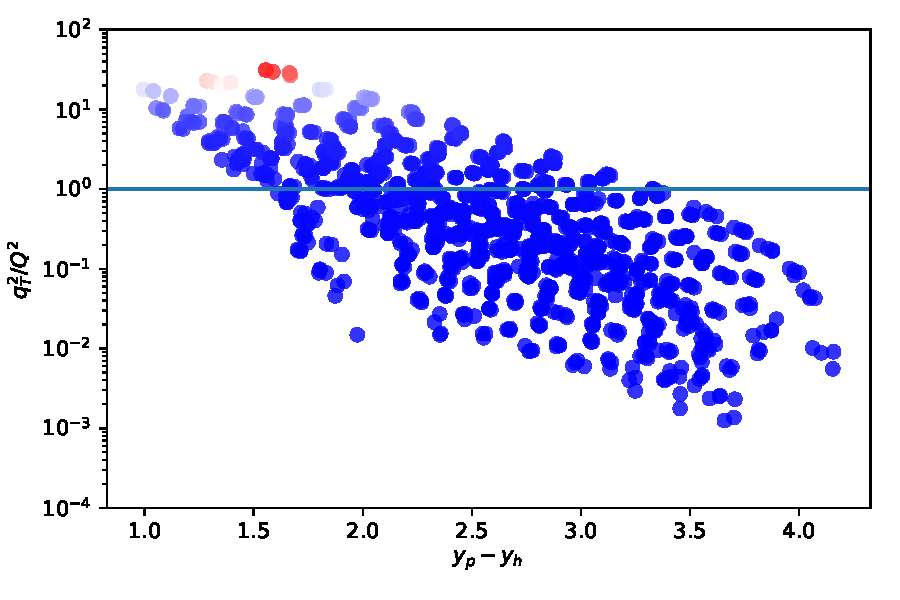
\includegraphics[width=0.45\textwidth]{\FigPath/hermes_data_all.pdf}
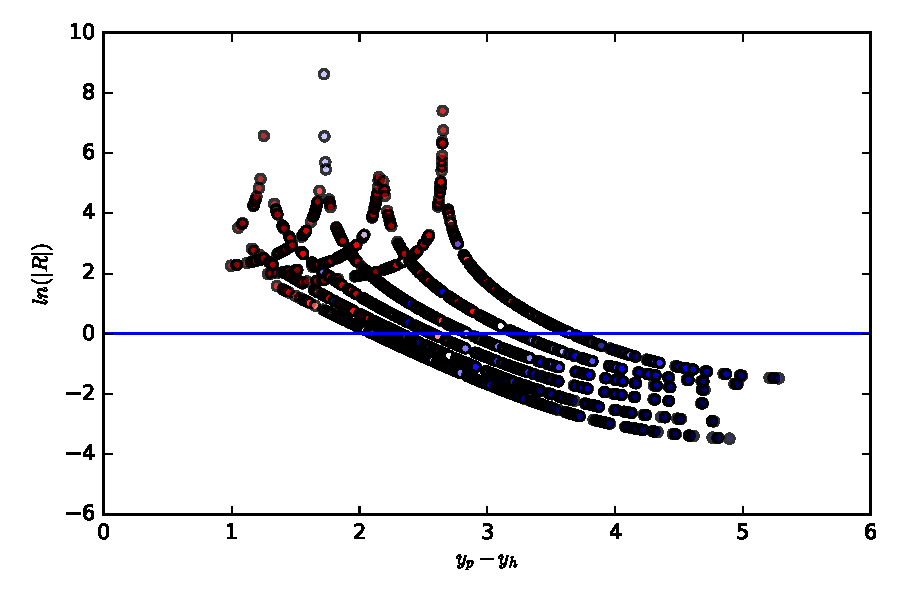
\includegraphics[width=0.45\textwidth]{\FigPath/hermes_data_all_lnR.pdf}
\caption{\label{Fig:hermes_data_rapidity}
[Color online]  {\bf Left panel:} Scatter plot of $q_T^2/Q^2$ vs $y_p-y_h$ for HERMES multiplicity data.  The solid line corresponds to $q_T^2/Q^2=1$. {\bf Right panel:} Scatter plot of $q_T^2/Q^2$  vs $\ln|R|$ for HERMES multiplicity data. Red (deep blue) color in the plots corresponds to growing (diminishing) values of $q_T^2/Q^2$.
}
\end{figure}
%%%%%%%%%

%%%%%%%%%
\begin{figure}[htb!]
\centering
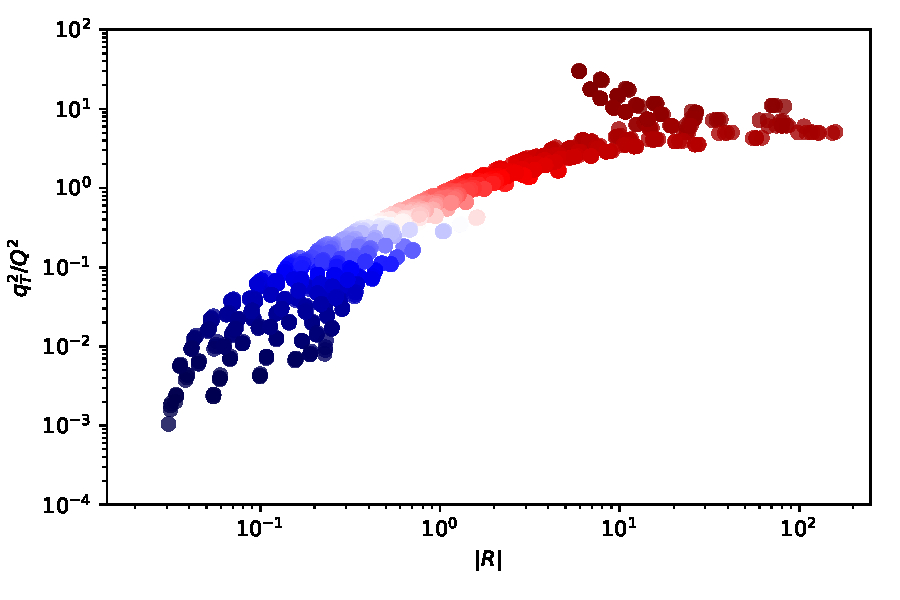
\includegraphics[width=0.45\textwidth]{\FigPath/hermes_data_pion_qt_vs_R.pdf}
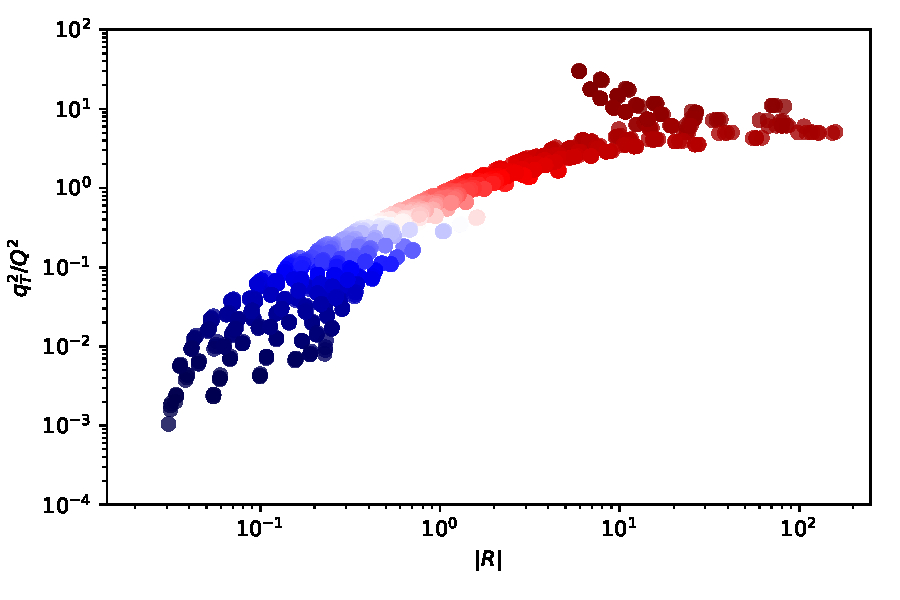
\includegraphics[width=0.45\textwidth]{\FigPath/hermes_data_kaon_qt_vs_R.pdf}
\caption{\label{Fig:hermes_data_qt_vs_R}
[Color online] {\bf Left panel:} Scatter plot of $q_T^2/Q^2$ vs $|R|$ for $\pi^\pm$ HERMES multiplicity data . {\bf Right panel:} 
Scatter plot of $q_T^2/Q^2$ vs $|R|$ for $K^\pm$ HERMES multiplicity data . Red (deep blue) color in the plots corresponds to growing (diminishing) values of $q_T^2/Q^2$.
}
\end{figure}
%%%%%%%%%
The scatter plot of  $q_T^2/Q^2$ vs $y_p-y_h$ for HERMES multiplicity data is shown in Fig.~\ref{Fig:hermes_data_rapidity}. In order to interpret the data in terms of TMD factorization, one must ensure applicability of factorization and make sure that the production mechanism corresponds to the ``beam" fragmentation. One requirement is $q_T \ll Q$. One can see from Fig.~\ref{Fig:hermes_data_rapidity} that  $q_T^2/Q^2$ for HERMES data can reach high values, and indeed 799 points are such that $q_T^2/Q^2>1$. Ref.~\cite{Boglione:2016bph} proposes collinearity, $R$, as a filter to  safely separate the ``forward'' and ``backward'' rapidity regions and ensure ``beam" fragmentation. One can also see from the right panel of Fig.~\ref{Fig:hermes_data_rapidity}  that values of $q_T^2/Q^2$ HERMES are correlated with values of $|R|$.
The exact starting value of $q_T^2/Q^2$ when the TMD factorization should become appropriate is not exactly known and should be determined phenomenologically. In order to be able to describe SIDIS cross section in a wide region of $q_T$ one should use the so-called $W+Y$ prescription, see for instance Ref.~\cite{Collins:2016hqq}, however at present for SIDIS data there are difficulties in implementation of this prescription, see Ref.~\cite{Gonzalez-Hernandez:2018ipj}. In this study we will use only TMD approximated cross-section as in Eq.~\eqref{e:dsigma} and consequently multiplicity as in Eq.~\eqref{e:mult_HERMES}.

We can state that if one imposes $R<1$-cut, then {\em simultaneously}  $q_T^2/Q^2$ are cut to smaller values $q_T^2/Q^2<1$, see left panel of Fig.~\ref{Fig:hermes_data_rapidity}. The same statement is true only to some extent for the cut in $y_p-y_h$, as only for large rapidity separation $y_p-y_h > 3.5$ the values of $q_T^2/Q^2$ become smaller than 1.  Fig.~\ref{Fig:hermes_data_R} shows $|R|$ versus $y_p-y_h$, and $\ln|R|$ versus $y_p-y_h$.
%%%%%%%%%
\begin{figure}[htb!]
\centering
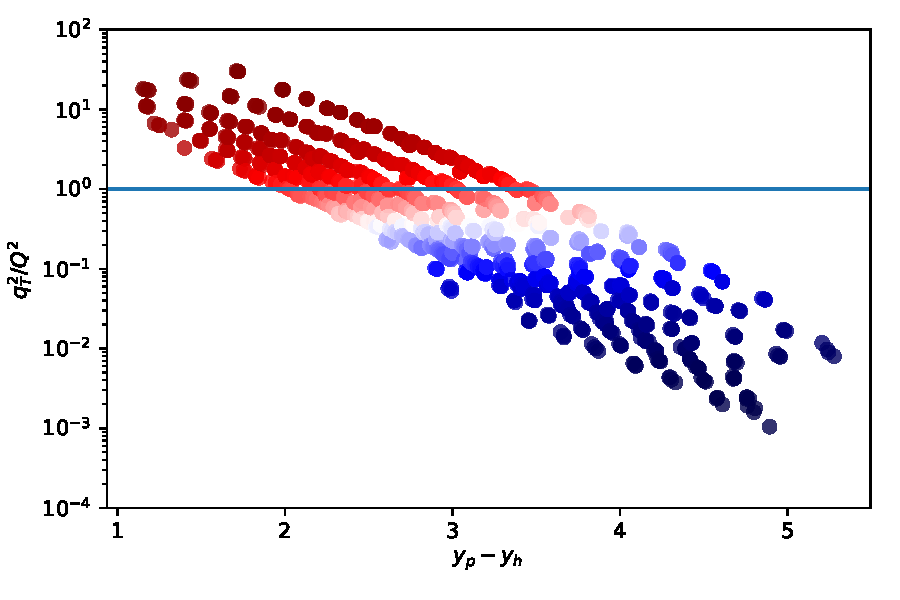
\includegraphics[width=0.45\textwidth]{\FigPath/hermes_data_pion.pdf}
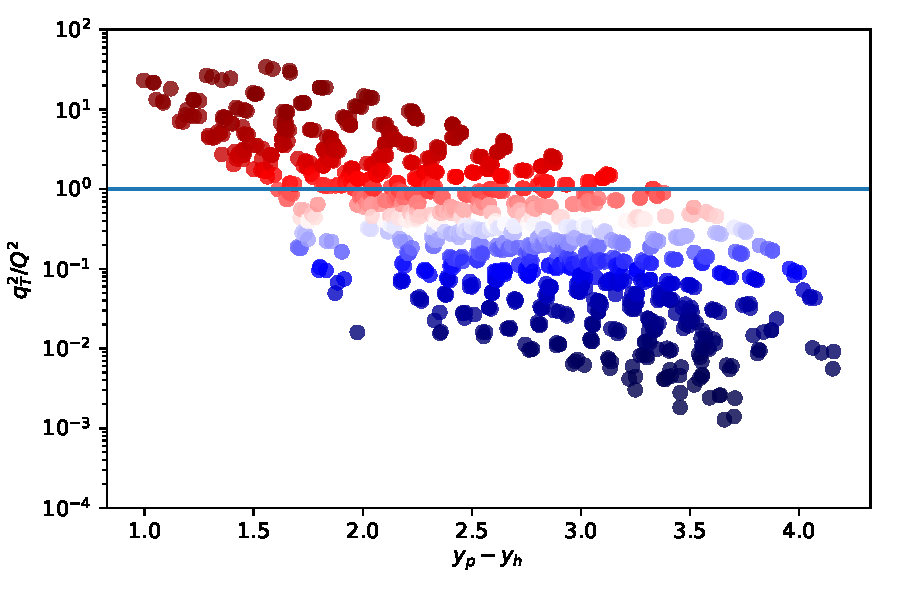
\includegraphics[width=0.45\textwidth]{\FigPath/hermes_data_kaon.pdf}
\caption{\label{Fig:hermes_data_R}
[Color online] {\bf Left panel:} Scatter plot of $q_T^2/Q^2$ vs $y_p-y_h$ for $\pi^\pm$ HERMES multiplicity data . {\bf Right panel:} 
Scatter plot of $q_T^2/Q^2$ vs $y_p-y_h$ for $K^\pm$ HERMES multiplicity data . The solid line corresponds to $R=1$. Red (deep blue) color in the plots corresponds to growing (diminishing) values of $q_T^2/Q^2$.
}
\end{figure}
%%%%%%%%%
One can see from Fig.~\ref{Fig:hermes_data_R} that lower values of $|R|$ are correlated with higher values of $y_p-y_h$, one can also see that $|R|$ becomes very large for low values of $y_p-y_h$. The distinct families of curves in Fig.~\ref{Fig:hermes_data_R} correspond to 8 bins in $x_B$ of HERMES data. For a given bin in $x_B$ all data for different hadron types, different targets, values of $z_h$, $Q^2$, and $P_{hT}$ belong to a particular distinct curve.

%If we make an assumption that the proton and the produced hadron are separated by a sufficiently large rapidity interval, and the initial quark rapidity is close to the proton rapidity $|y_i - y_p| \ll |y_p|$ and the final quark has approximately the same rapidity as the pion $|y_f -y_h| \ll |y_h|$, then we obtain
%\begin{equation}
%R \sim \frac{e^{y_p-y_h}} {e^{2 (y_p-y_h)}-1}\,\to \frac{1} {e^{y_p-y_h}}
%\label{eq:r_mod}
%\end{equation}
if% $y_p-y_h$ is large enough, so that $e^{y_p-y_h} \gg 1$ and $R \ll 1$. 
One can see that $R$ is an exponential measure, so we will introduce an R-filter using $\ln R < A$ instead of $R < A$, where $A < 1$. We also deduce that a simpler filter to ensure the collinearity is $y_p-y_h > A$, where $A> 1$ is sufficiently large. In practice our assumptions that lead to Eq.~\eqref{eq:r_mod} are not always satisfied for all HERMES data, see %Fig.~\ref{Fig:hermes_torino_rapidity}, however in the region of interest (negative rapidities for produced hadrons) these assumptions are reasonable.
%%%%%%%%%
%\begin{figure}[htb!]
%\centering
%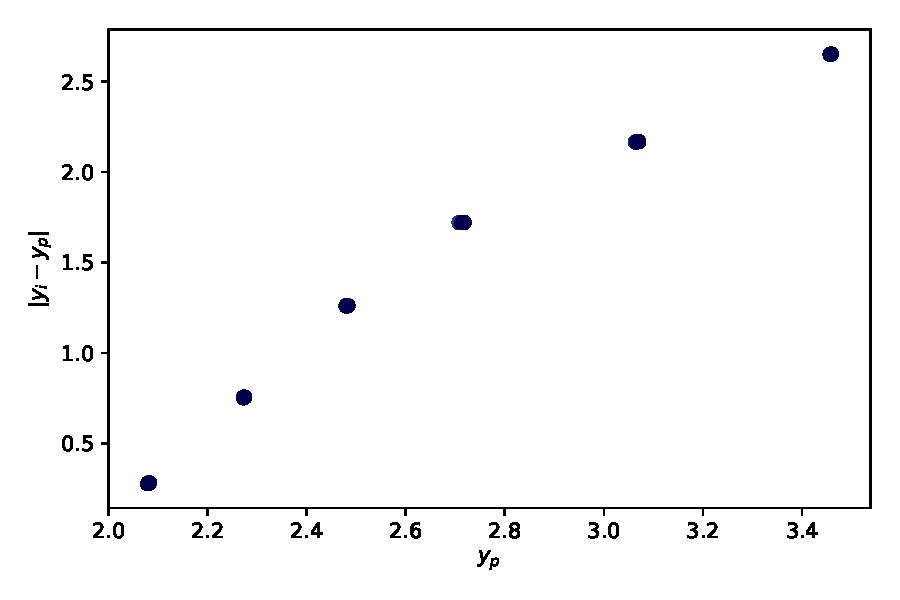
\includegraphics[width=0.45\textwidth]{\FigPath/hermes_data_yi_minus_yp.pdf}
%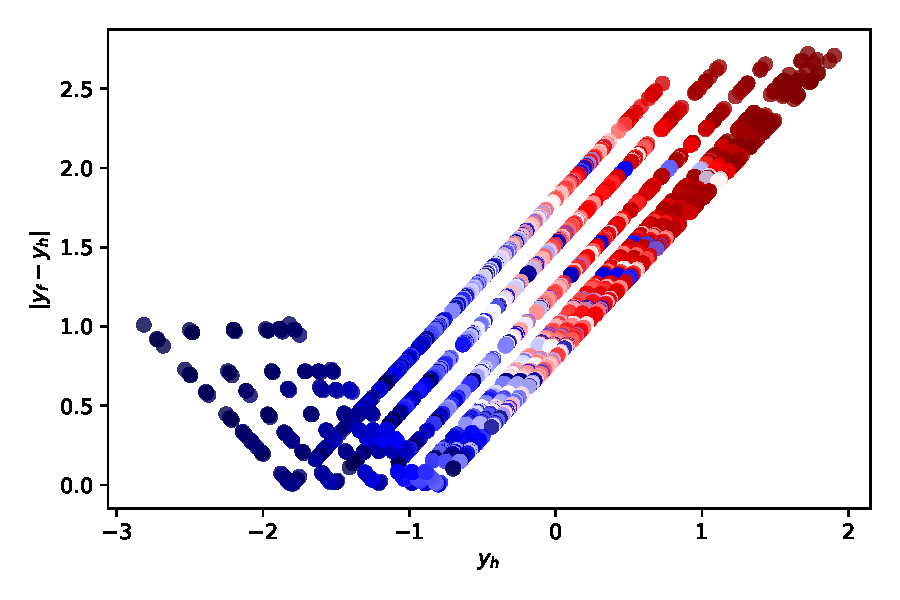
\includegraphics[width=0.45\textwidth]{\FigPath/hermes_data_yf_minus_yh.pdf}
%\caption{\label{Fig:hermes_torino_rapidity}
%[Color online] {\bf Left panel:} Scatter plot of $y_i-y_p$ vs $y_p$ for HERMES multiplicity data . {\bf Right panel:} 
%Scatter plot of HERMES multiplicity data $y_i-y_h$ vs $y_h$. Red (deep blue) color in the plots corresponds to growing (diminishing) values of $q_T^2/Q^2$
%}
%\end{figure}
%%%%%%%%%

Let us discuss first the application of the ``standard'' cut from Eq.~\eqref{e:st_cut}. As shown in Ref.~\cite{Anselmino:2013lza} the data filtered by Eq.~\eqref{e:st_cut} can be described well in the framework of TMD parton model. The cut of Eq.~\eqref{e:st_cut} however does not necessarily ensure filtering the data for which TMD factorization is applicable, moreover, as pointed out in Ref.~\cite{Boglione:2016bph} it does not ensure filtering of the data in the ``beam" fragmentation region. In order to demonstrate it, let us plot $q_T^2/Q^2$ versus $y_p-y_h$ in Fig.~\ref{Fig:hermes_torino}.
%%%%%%%%%
\begin{figure}[htb!]
\centering
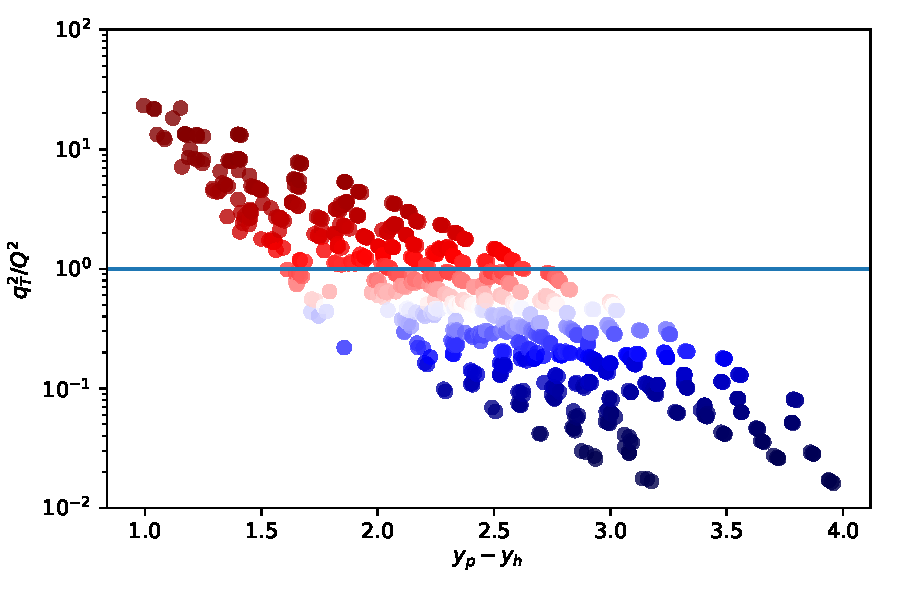
\includegraphics[width=0.45\textwidth]{\FigPath/hermes_data_torino.pdf}
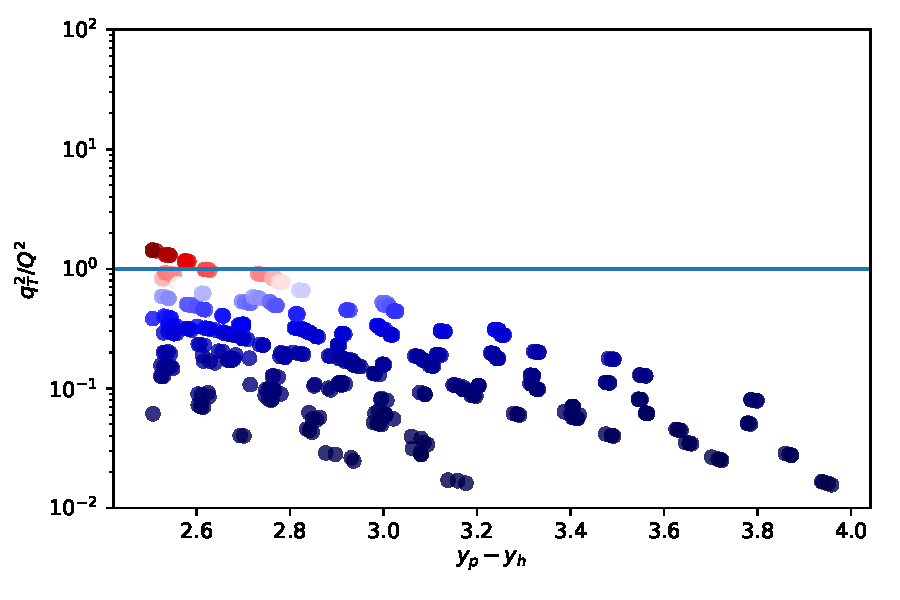
\includegraphics[width=0.45\textwidth]{\FigPath/hermes_data_torino_rapidity.pdf}
\caption{\label{Fig:hermes_torino}
[Color online] {\bf Left panel:} Scatter plot of $q_T^2/Q^2$ vs $y_p-y_h$ for HERMES multiplicity data filtered by the ``standard'' cut from Eq.~\eqref{e:st_cut}. {\bf Right panel:} 
Scatter plot of HERMES multiplicity data filtered by the ``standard'' cut from Eq.~\eqref{e:st_cut1} and $y_p-y_h>2.5$. The solid line corresponds to $q_T^2/Q^2=1$. Red (deep blue) color in the plots corresponds to growing (diminishing) values of $q_T^2/Q^2$.
}
\end{figure}
%%%%%%%%%
One can see from Fig.~\ref{Fig:hermes_torino} that $q_T^2/Q^2$ can reach high values, even though one should ensure that $q_T^2/Q^2\ll 1$ for the applicability of TMD factorization. In case of HERMES multiplicities, cuts from Eq.~\eqref{e:st_cut} result in total of 978 points and 292 points are such that $q_T^2/Q^2>1$. On the other hand, if we add $y_p-y_h>2.5$ selection criteria to Eq.~\eqref{e:st_cut}, then only 11 out of 473 points are such that $q_T^2/Q^2>1$. In order to study the influence of restriction of the rapidity interval on the results of the fit, we will use cuts from Eq.~\eqref{e:st_cut} and add $y_p-y_h>A$ selection criteria, where $A \in[1.25, 3.5]$:
\begin{equation}
z_h < 0.6 \quad\quad Q^2 > 1.69 \; \textrm{GeV}^2  
\quad\quad 0.2 < P_{hT} < 0.9 \; \textrm{GeV} \quad\quad y_p-y_h > A  \quad\quad\quad{\rm (new\;standard\;cut)}\,.\label{e:st_cut1}
\end{equation}
An example of such data selection for A = 2.5 is shown in the right panel of Fig.~\ref{Fig:hermes_torino}.

The second set of cuts that we will explore will be motivated by ensuring applicability of TMD factorization together with selection of large rapidity interval, we will call it ``rapidity" cut:
\begin{equation}
z_h > 0.2 \quad\quad  z_h < 0.6 \quad\quad Q^2 > 1.69 \; \textrm{GeV}^2  
\quad\quad  q_T^2/Q^2 < \, 0.15   \quad\quad y_p-y_h > A \quad\quad{\rm (rapidity\;cut)}\,.\label{e:rapidity_cut}
\end{equation}
Notice that we cut the values of $z_h<0.2$, Ref.~\cite{schnell}. We will vary the value $A \in[1.25, 3.5]$ in order to test the sensitivity of the fit results to this value. Scatter plot of the filtered data by the rapidity cut from Eq.~\eqref{e:rapidity_cut} is shown in Fig.~\ref{Fig:hermes_new}.

%%%%%%%%%
\begin{figure}[htb!]
\centering
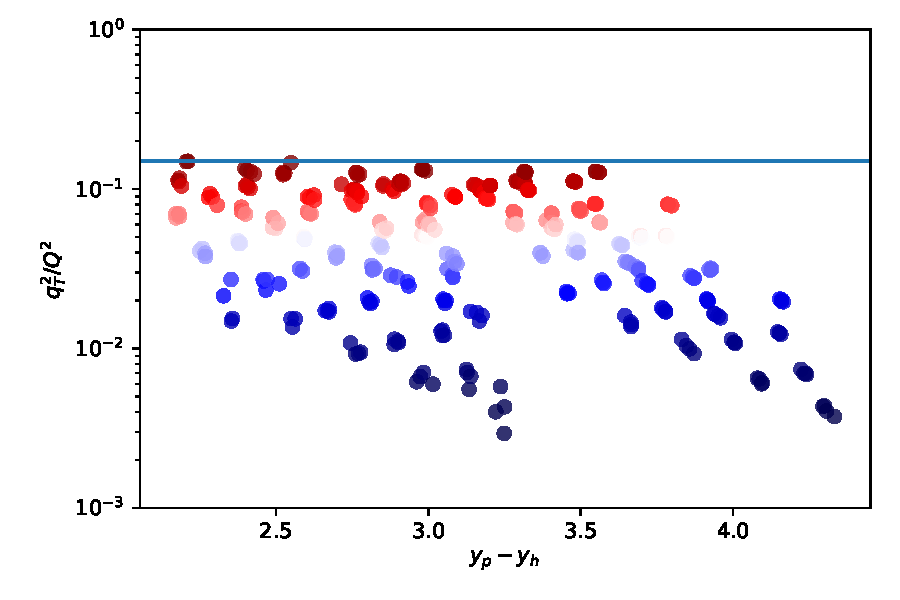
\includegraphics[width=0.45\textwidth]{\FigPath/hermes_data_rapidity.pdf}
\caption{\label{Fig:hermes_new}
[Color online] Scatter plot of HERMES multiplicity data filtered by the rapidity cut from Eq.~\eqref{e:rapidity_cut}. The solid line corresponds to $q_T^2/Q^2=0.15$. Red (deep blue) color in the plots corresponds to growing (diminishing) values of $q_T^2/Q^2$.
}
\end{figure}
%%%%%%%%%

The third set of cuts that we will explore will include collinearity criteria from Ref.~\cite{Boglione:2016bph}, we will discard any data for large values of $|R|$, we will call it R-cut: 
 \begin{equation}
z_h > 0.2 \quad\quad  z_h < 0.6 \quad\quad Q^2 > 1.69 \; \textrm{GeV}^2  
\quad\quad   \ln |R|  < A \quad\quad{\rm (R\;cut)}\,.\label{e:r_cut}
\end{equation}
We will vary the value $A \in[-0.5, -2.5]$ in order to test the sensitivity of the fit results to this value. The scatter plot of HERMES multiplicity data filtered by the R-cut from Eq.~\eqref{e:r_cut},  $\ln |R|  < -0.5$ and $\ln |R| < -2.5$, is shown in Fig.~\ref{Fig:hermes_R}. One can see that $\ln |R|  < -0.5$ ensures selection of $q_T^2/Q^2<1$. One can also see from Fig.~\ref{Fig:hermes_R}, that filtering larger negative values of $\ln |R|$ correspond to simultaneous filtering out smaller values of $y_p - y_h$, and large values of $q_T^2/Q^2$ (compare left and right panels of Fig.~\ref{Fig:hermes_R}).
 
 %%%%%%%%%
\begin{figure}[htb!]
\centering
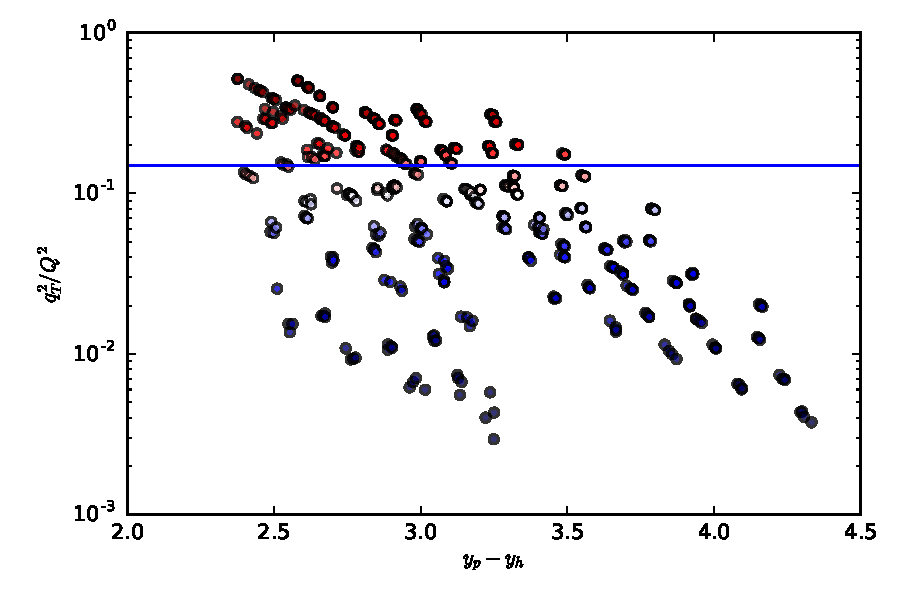
\includegraphics[width=0.45\textwidth]{\FigPath/hermes_data_R.pdf}
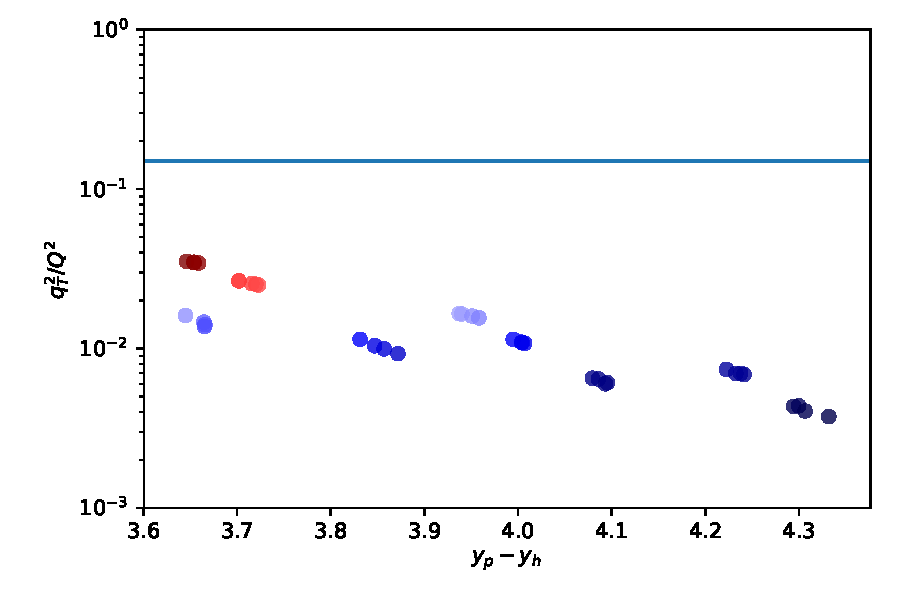
\includegraphics[width=0.45\textwidth]{\FigPath/hermes_data_R25.pdf}
\caption{\label{Fig:hermes_R}
[Color online] {\bf Left panel:} Scatter plot of HERMES multiplicity data filtered by the R-cut from Eq.~\eqref{e:r_cut},  $\ln R  < -0.5$. {\bf Right panel:} Scatter plot of HERMES multiplicity data filtered by the R-cut from Eq.~\eqref{e:r_cut},  $\ln R  < -2.5$. The solid line corresponds to $q_T^2/Q^2=0.15$. Red (deep blue) color in the plots corresponds to growing (diminishing) values of $q_T^2/Q^2$.
}
\end{figure}
%%%%%%%%%
 

 
If one compares right panel of Fig.~\ref{Fig:hermes_torino},  Fig.~\ref{Fig:hermes_new}, and Fig.~\ref{Fig:hermes_R}, it is easy to see that data selections are quite similar, and thus we expect that fit results will be similar. We fit the (flavor-dependent) Gaussian widths to the the multiplicities using Eq.~(\ref{e:mult_HERMES}) (along with (\ref{e:avg_kT})).  The details of this extraction and the results for our parameters will be discussed in the next section.





\subsection{Fit and Results}
\label{s:fit}
We will use the following collinear functions in our analysis: PDFs are CJ15LO from Ref.~\cite{Accardi:2016qay}, FFs are  the DSS LO FF set
from Ref.~\cite{deFlorian:2007aj}. The value of initial scale $Q_0$ will always coincide with the lowest $Q^2$ cut-off in our cuts: $Q_0^2 = 1.69$ (GeV$^2$). We will make the following assumptions on the intrinsic non perturbative parameters:
For the transverse-momentum widths $\langle k_\perp^2 \rangle_q$ of the TMD PDFs, two Gaussian widths are used, one for the
  valence type $\langle k_\perp^2 \rangle_{val}$ ($q=u, d$) and one for the
  sea-quark type $\langle k_\perp^2 \rangle_{sea}$ ($q = \bar u, \bar d, s, \bar s$) functions.
Similarly, for the TMD FFs two Gaussian widths for $\langle p_\perp^2 \rangle_q$
are used, for the favored (such as $u$ or $\bar d$ to $\pi^+$) and
unfavored ($\bar u$ or $d$ to $\pi^+$) type of FF. We have separate favored and unfavored widths for pion and Kaon fragmentation TMDs.
Finally, we also fit $g_{K_0}$ that encodes non perturbative TMD evolution.
%
In total, we therefore have 7 parameters to be extracted
from HERMES data.
%
The theoretical expectation from the chiral soliton
model~\cite{Schweitzer:2012hh} is to have a larger sea-quark width compared to valence quark width, so that $\langle k_\perp^2 \rangle_{sea}/\langle k_\perp^2 \rangle_{val}\sim 5$.
%
Extraction of parameters and error analysis will be performed by using Monte Carlo techniques \cite{Sato:2016tuz,Sato:2016tuz} developed by Jefferson Lab JAM Collaboration~\cite{JAM}.
Using the nested sampling MC algorithm~\cite{Skilling:2004,
Mukherjee:2005wg, Shaw:2007jj}, we compute the expectation
value E[${\cal O}$] and variance V[${\cal O}$],
%
\begin{subequations}
\label{eq:EV}
\begin{eqnarray}
\hspace*{-0.5cm}
{\rm E}[{\cal O}]
&=& \int d^n a\, {\cal P}({\bm a}|{\rm data})\,
    {\cal O}({\bm a})\
\simeq\ \sum_k w_k\, {\cal O}({\bm a_k}),			\\
%
\hspace*{-0.5cm}
{\rm V}[{\cal O}]
&=& \int d^n a\, {\cal P}({\bm a}|{\rm data})
    \big( {\cal O}({\bm a}) - {\rm E[{\cal O}]} \big)^2		\notag\\
&\simeq& \sum_k w_k
	 \big( {\cal O}({\bm a_k}) - {\rm E[{\cal O}]} \big)^2,
\end{eqnarray}
\end{subequations}%
%
for each observable ${\cal O}$ (such as a TMD or a function of TMDs),
which is a function of the $n$-dimensional vector parameters ${\bm a}$
with probability density ${\cal P}({\bm a}|{\rm data})$
\cite{Sato:2016wqj}.
Using Bayes' theorem, the latter is given by
%
\begin{eqnarray}
{\cal P}({\bm a}|{\rm data})
&=& \frac{1}{Z}\, {\cal L}({\rm data}|{\bm a})\, \pi({\bm a}),
\end{eqnarray}
%
where $\pi({\bm a})$ is the prior distribution for the vector
parameters ${\bm a}$, and
%
\begin{eqnarray}
{\cal L}({\rm data}|{\bm a})
&=& \exp\left[ -\frac12 \chi^2({\bm a}) \right]
\end{eqnarray}
%
is the likelihood function, with
  $Z = \int d^n a\, {\cal L}({\rm data}|{\bm a})\, \pi({\bm a})$
the Bayesian evidence parameter.
%
Using a flat prior, the nested sampling algorithm constructs a set
of MC samples $\{\bm a_k\}$ with weights $\{w_k\}$, which are then
used to evaluate observables.



Resulting parameters of the fits with  the  new ``standard'' cut from Eq.~\eqref{e:st_cut1} 
are shown in Fig.~\ref{Fig:torino}.

%%%%%%%%%
\begin{figure}[htb!]
\centering
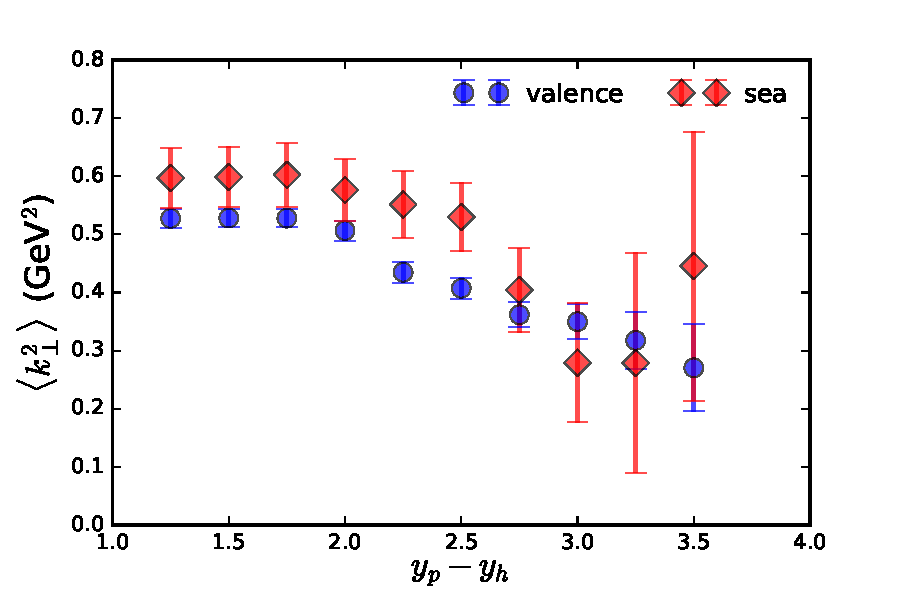
\includegraphics[width=0.45\textwidth]{\FigPath/kt_dy_torino.pdf}{\tiny(a)}%
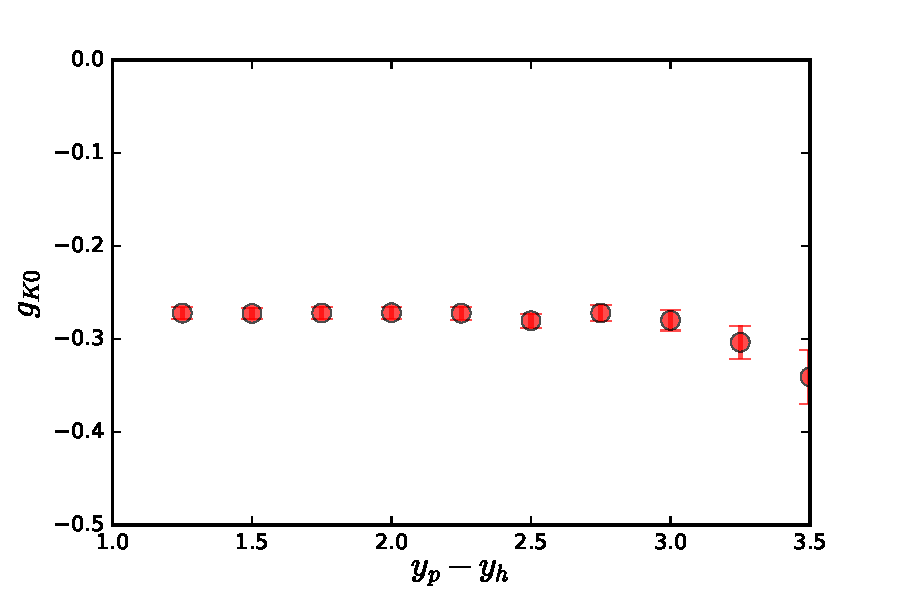
\includegraphics[width=0.45\textwidth]{\FigPath/gk0_dy_torino.pdf}{\tiny(b)}\\% 
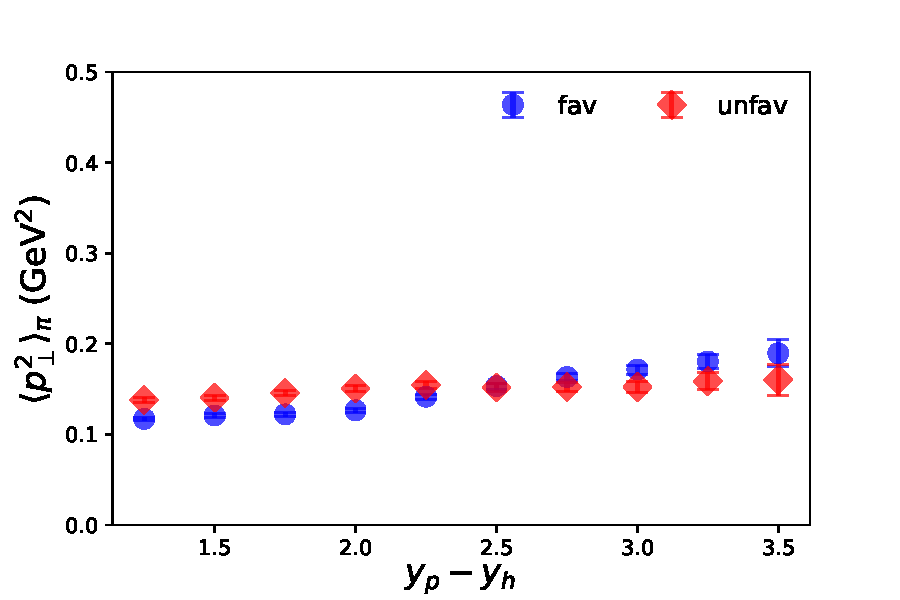
\includegraphics[width=0.45\textwidth]{\FigPath/pt_pion_dy_torino.pdf}{\tiny(c)}%
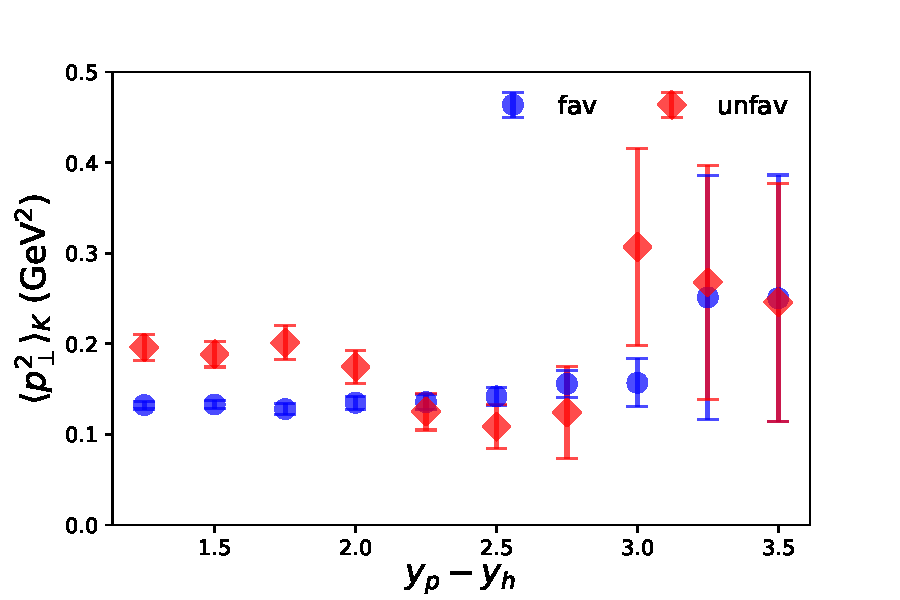
\includegraphics[width=0.45\textwidth]{\FigPath/pt_kaon_dy_torino.pdf}{\tiny(d)}%
\caption{\label{Fig:torino}
Fitted parameters of the model with cuts from Eq.~\eqref{e:st_cut1} as function of $y_p-y_h$. (a) $\langle k_\perp^2 \rangle_a$ for valence and sea quarks,
(b) $g_{K_0}$,
(c) $\langle p_\perp^2 \rangle_a$ for pion favored and unfavored fragmentation, (d) $\langle p_\perp^2 \rangle_a$ for Kaon favored and unfavored fragmentation.
}
\end{figure}
%%%%%%%%%

[Comments, discussions....]
\newpage
Resulting parameters of the fits with  the ``rapidity'' cut from Eq.~\eqref{e:rapidity_cut} 
are shown in Fig.~\ref{Fig:rapidity_cut}.
%%%%%%%%%
\begin{figure}[htb!]
\centering
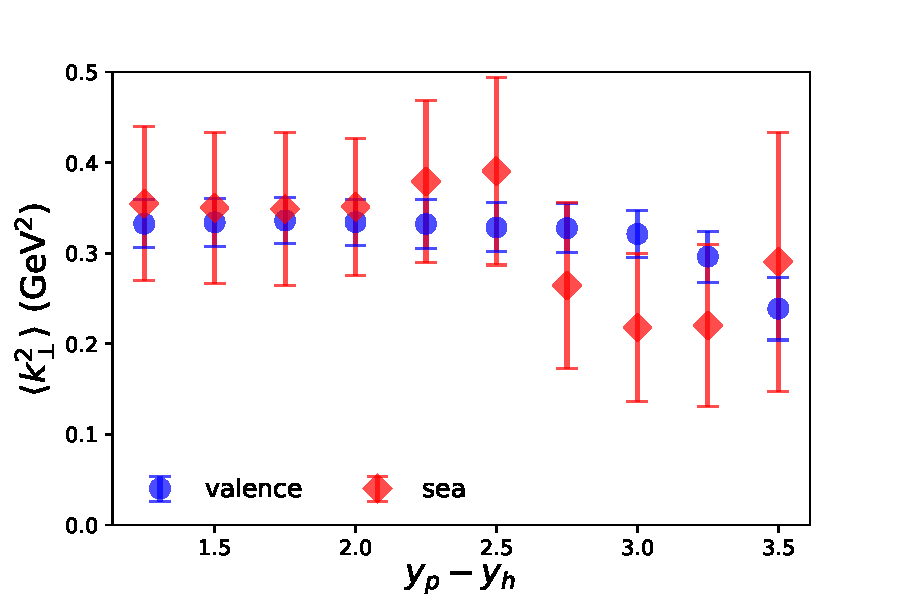
\includegraphics[width=0.45\textwidth]{\FigPath/kt_dy_alexei.pdf}{\tiny(a)}%
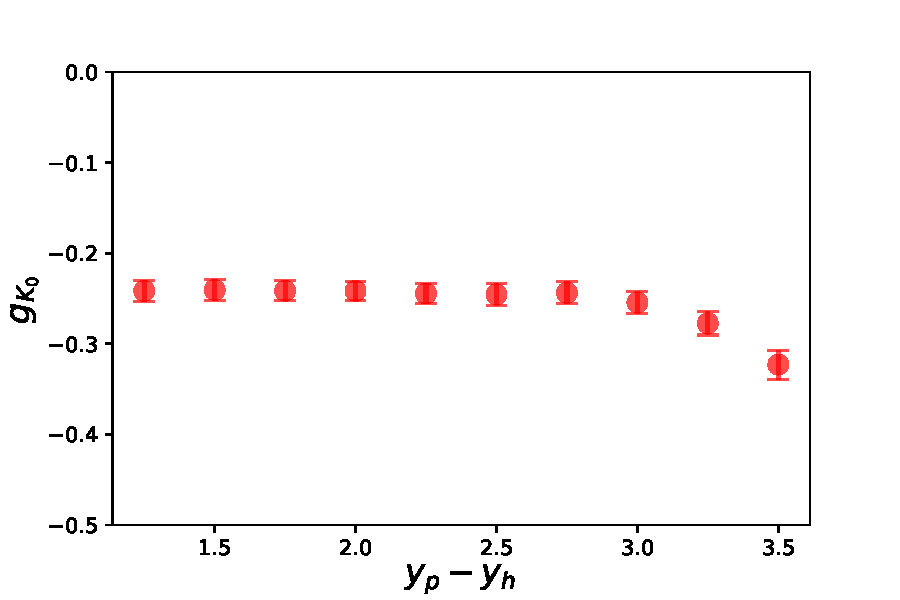
\includegraphics[width=0.45\textwidth]{\FigPath/gk0_dy_alexei.pdf}{\tiny(b)}\\% 
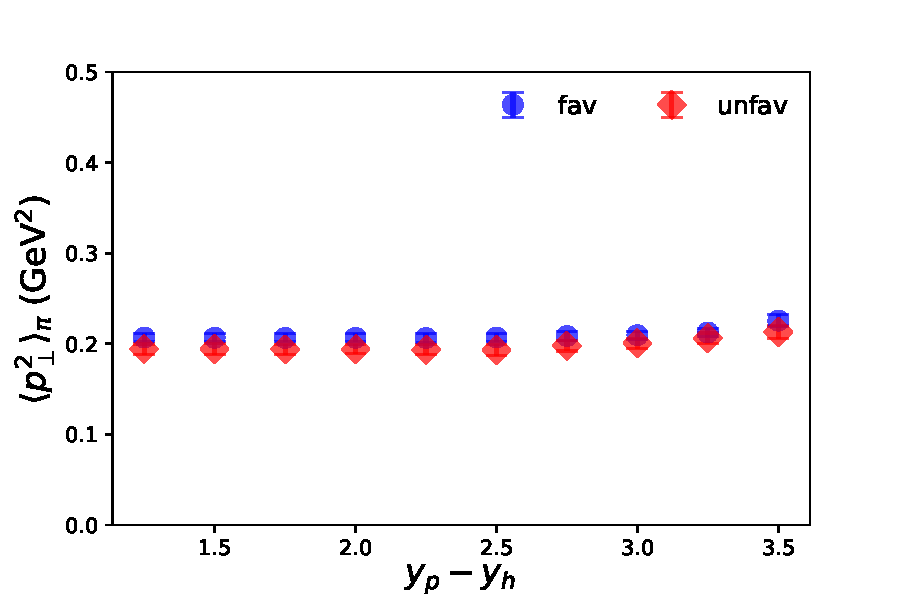
\includegraphics[width=0.45\textwidth]{\FigPath/pt_pion_dy_alexei.pdf}{\tiny(c)}%
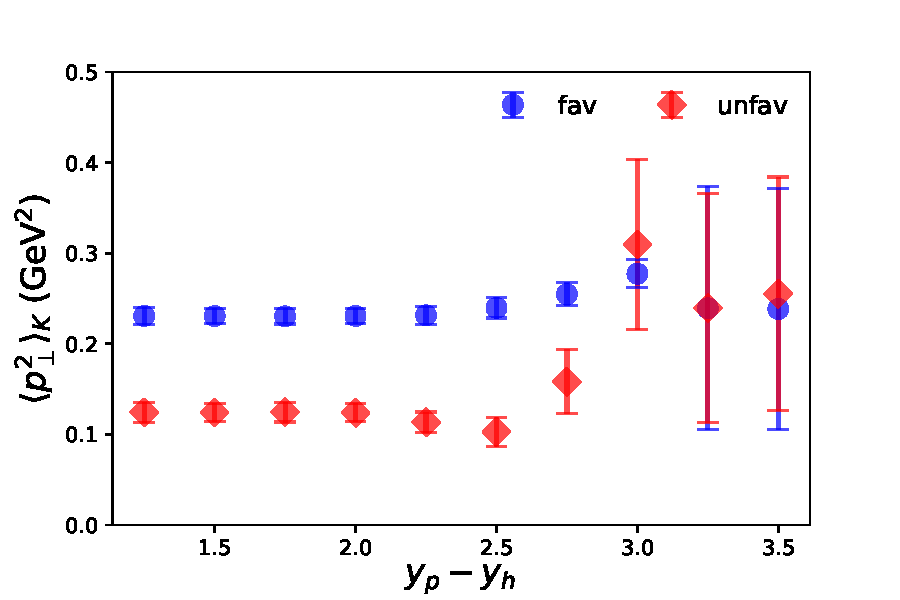
\includegraphics[width=0.45\textwidth]{\FigPath/pt_kaon_dy_alexei.pdf}{\tiny(d)}%
\caption{\label{Fig:rapidity_cut}
Fitted parameters of the model with cuts from Eq.~\eqref{e:rapidity_cut} as function of $y_p-y_h$. (a) $\langle k_\perp^2 \rangle_a$ for valence and sea quarks,
(b) $g_{K_0}$,
(c) $\langle p_\perp^2 \rangle_a$ for pion favored and unfavored fragmentation, (d) $\langle p_\perp^2 \rangle_a$ for Kaon favored and unfavored fragmentation.
}
\end{figure}

[Comments, discussions....]
\newpage


Resulting parameters of the fits with  the R-cut from Eq.~\eqref{e:r_cut} 
are shown in Fig.~\ref{Fig:r_cut}.
%%%%%%%%%
\begin{figure}[htb!]
\centering
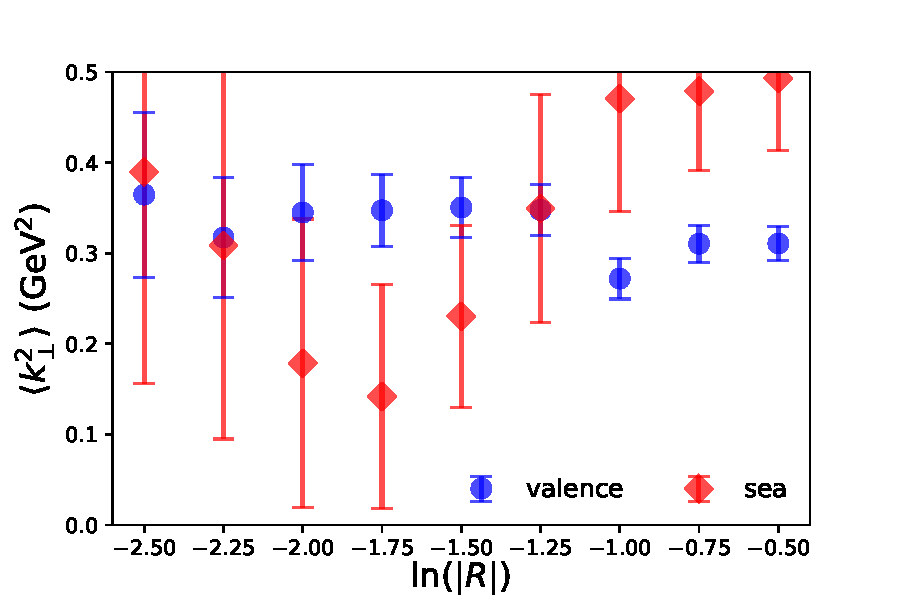
\includegraphics[width=0.45\textwidth]{\FigPath/kt_R_alexei.pdf}{\tiny(a)}%
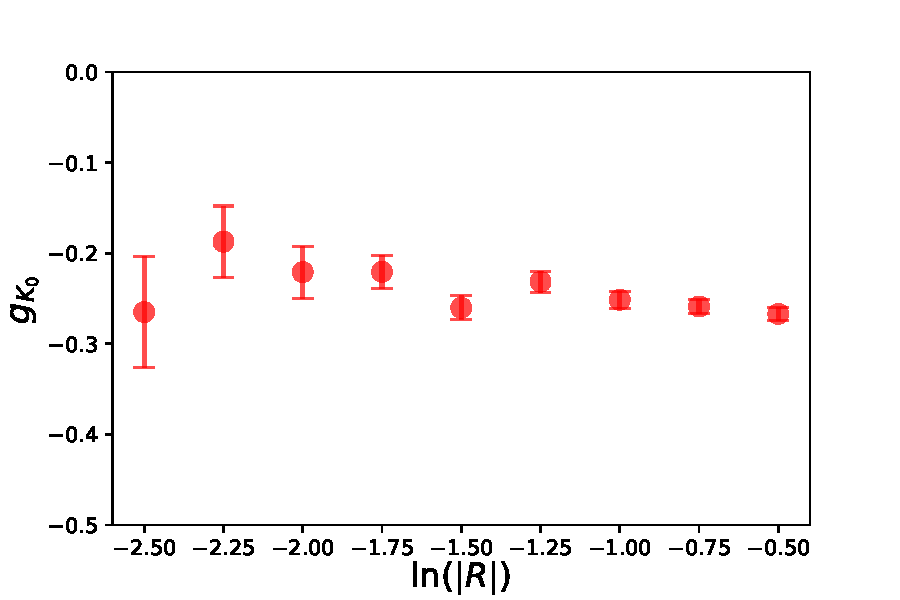
\includegraphics[width=0.45\textwidth]{\FigPath/gk0_R_alexei.pdf}{\tiny(b)}\\% 
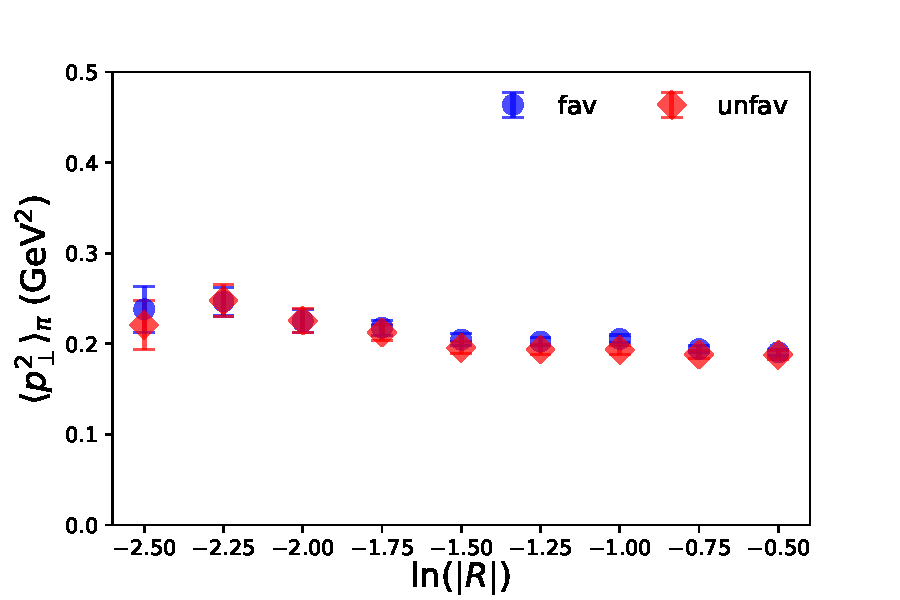
\includegraphics[width=0.45\textwidth]{\FigPath/pt_pion_R_alexei.pdf}{\tiny(c)}%
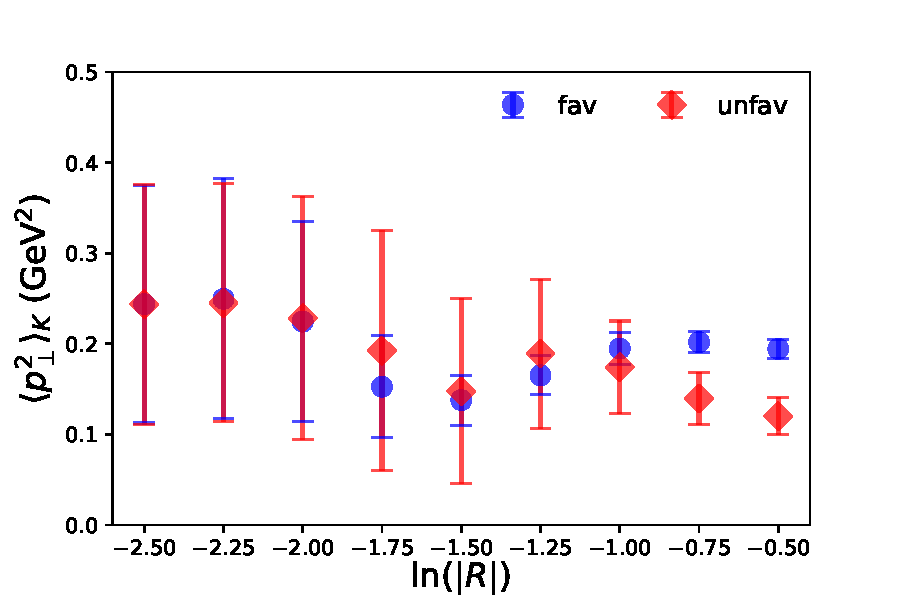
\includegraphics[width=0.45\textwidth]{\FigPath/pt_kaon_R_alexei.pdf}{\tiny(d)}%
\caption{\label{Fig:r_cut}
Fitted parameters of the model with cuts from Eq.~\eqref{e:r_cut} as function of $\ln(|R|)$. (a) $\langle k_\perp^2 \rangle_a$ for valence and sea quarks,
(b) $g_{K_0}$,
(c) $\langle p_\perp^2 \rangle_a$ for pion favored and unfavored fragmentation, (d) $\langle p_\perp^2 \rangle_a$ for Kaon favored and unfavored fragmentation.
}
\end{figure}

[Comments, discussions....]
\newpage


[Give details of fit: PDFs/FFs used, $\chi^2/d.o.f.$, error analysis, plots.]  In the end, we find the following Gaussian widths: $\langle k_\perp^2\rangle_{u_v} = 0.25\,{\rm GeV^2}$, $\langle p_\perp^2\rangle_{fav} = 0.17\,{\rm GeV^2}, \dots$.  These widths are consistent with an earlier extraction using high-energy EMC data~[CITE], where one would expect little impact from the R-cut given that the current and target fragmentation regions are well-separated in that case.  Therefore, we see the reduction in especially $\langle k_\perp^2\rangle$ found in Refs.~[CITE] is most likely due to ``contamination'' from data in the target fragmentation region.  Also, even though Ref.~[CITE] considers HERMES and COMPASS data, the majority of the data points used in that analysis are from high-energy $Z$-boson production at Fermi-lab.  Consequently, the widths found there are closer to the ones in this analysis since the ``contaminated'' HERMES and COMPASS data do not weigh heavily in the global analysis.  [Elaborate more.  Evolution effects?]


\section{Conclusions}
\label{s:concl}
[Summary of results.  Future work.  Impact moving forward.]



 
\section*{Acknowledgments}
The authors acknowledge useful conversations with Elena Boglione and Osvaldo Gonzalez during the early stages of this study.
 This material is based upon work supported by the
U.S. Department of Energy, Office of Science, Office of Nuclear
Physics under Award No. DE-FG02-07ER41460 (L.G.), No.~DE-AC05-06OR23177 (A.P.), by the National Science Foundation 
under Contract No. PHY-1623454 (A.P.), and within the 
framework of the TMD Topical Collaboration.

\bibliographystyle{h-physrev}
\bibliography{lg}
\end{document}
\endinput
%%%%%%%%%%%%%%%%%%%%%%%%%%%%%%%%%%%%%%%%%%%%%%%%%%%%%%%%%%%%%%%%%%%%%%%%





  
